 
\begin{frame}[plain]{Raspberry Pi}
	% this is a comment
	\begin{itemize}
		\item Raspberry Pi Version: Raspberry Pi 3
		\item Capable little computer that can be used for electronics projects
		\item Used to connect the camera with the nano-board for the line detection
	\end{itemize}
	
	\begin{figure}
	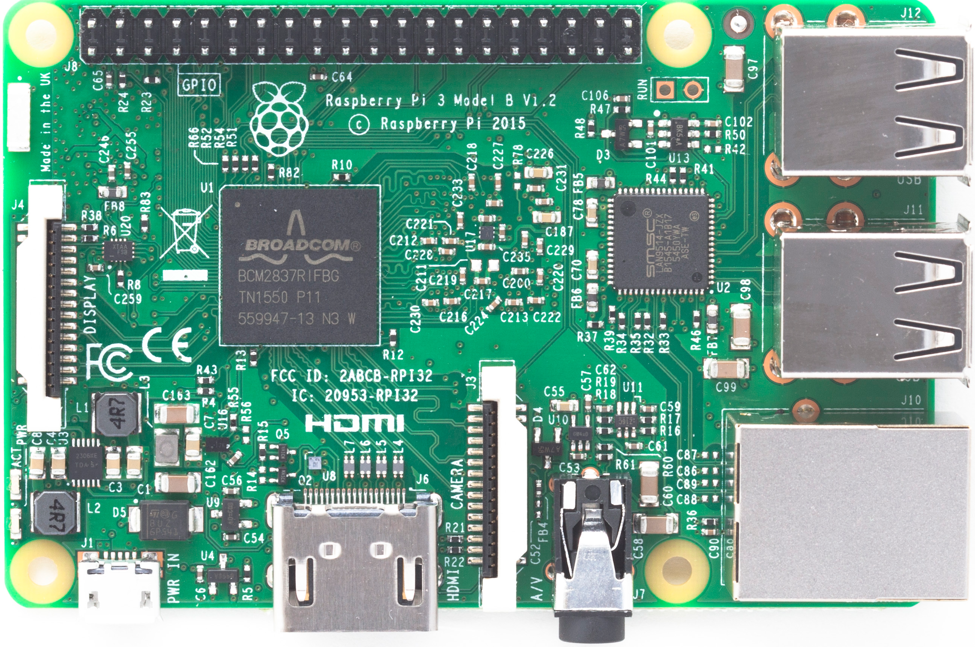
\includegraphics[width=7cm, height=5cm]{raspi.png}
	\end{figure}
	
	\vspace{2cm}
	this text has 2cm Distance from above (because of vspace)\\ % \\ means new line
	Abdallah
\end{frame}

\begin{frame}[plain]{Raspberry Pi}

Carried out steps:
\begin{enumerate}
		\item Raspbian installed (operating system for the Raspberry Pi)
		\item Connected to the laptop using Ethernet
		\item Used SSH (Secure Shell) to gain access to the command line of the Raspberry Pi
		\item Controlled the Raspberry Pi using VNC (a graphical desktop sharing system)
		\item Downloaded OpenCV and connected the camera
		\item Tested the Code for the line detection
	\end{enumerate}
	

	
To-Do:
\begin{enumerate}
		\item Connect the Raspberry Pi to the nano-board
		\item Align the line detection with the motor control
	\end{enumerate}

\end{frame}

\begin{frame}[plain]{Raspberry Pi}
\begin{figure}
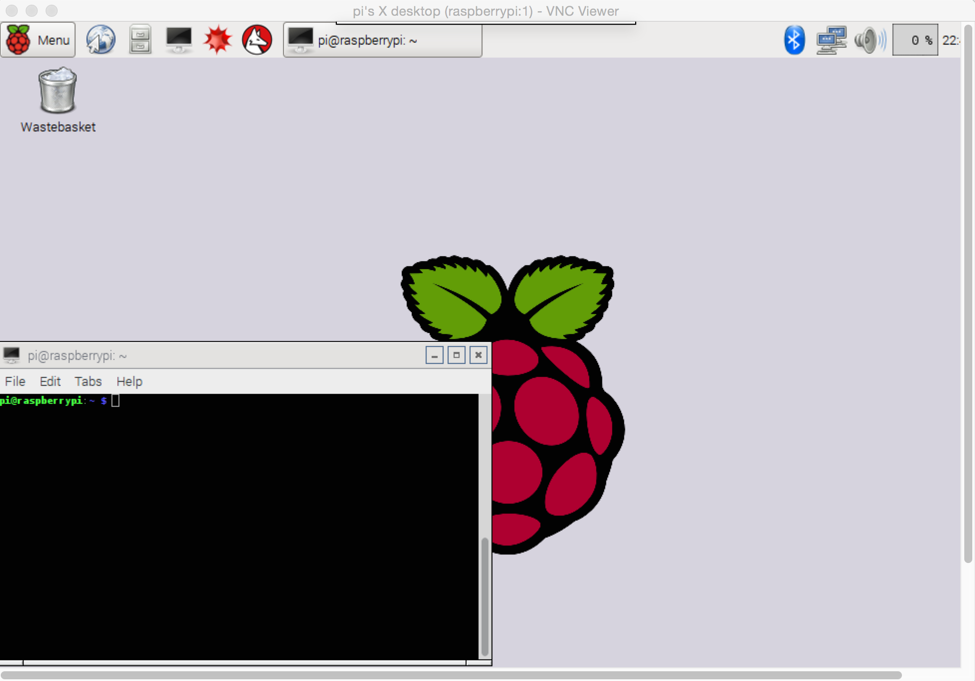
\includegraphics[width=8cm, height=7cm]{vnc.png}
\end{figure}	
\end{frame}